% SVN info for this file
%!TEX root = report.tex
\svnidlong
{$HeadURL$}
{$LastChangedDate$}
{$LastChangedRevision$}
{$LastChangedBy$}

\chapter{Load and DRES Modeling}
\labelChapter{model}

\begin{introduction}
  In this chapter, day-ahead modeling of loads and DRES production is explained. While the modeling done here is for the purpose of this Master's thesis alone, models based on the state of the art in prediction (\refChapterOnly{stateofart}) are envisaged to be developed in future.
\end{introduction}

\lettrine[nindent=0pt]{I}{n} order to construct load models for one full day, with a temporal resolution of one hour, two different initial models were chosen. They are based on the models found in \cite{Lopez2004} and \cite{Yin2009}. They describe typical load curves for one day, and based on them, two load curves (Model 1 and Model 2) are constructed.\refAppendixOnly{loaddresmodels} elaborates on the load and DRES models, with explanations regarding their formulation.

\section{Test Networks}

\lettrine[nindent=0pt]{T}{wo} different distribution networks, one urban, and one rural were tested using the developed algorithm. One is an urban network and the other is a rural network. The urban network, called the PREDIS network, is a test network present at G2E Lab/Grenoble INP, and its details are shown in \refFigureOnly{fig:predisnw}, refTableOnly{predisbase}, and \refTableOnly{predisImax}. The other network is shown in \refFigureOnly{fig:dasnw}, and its other details are shown in \refTableOnly{dasbase} and \refTableOnly{dasImax}.\\

\begin{table}[!h]
    \begin{minipage}[!h]{.65\textwidth}
	\centering
	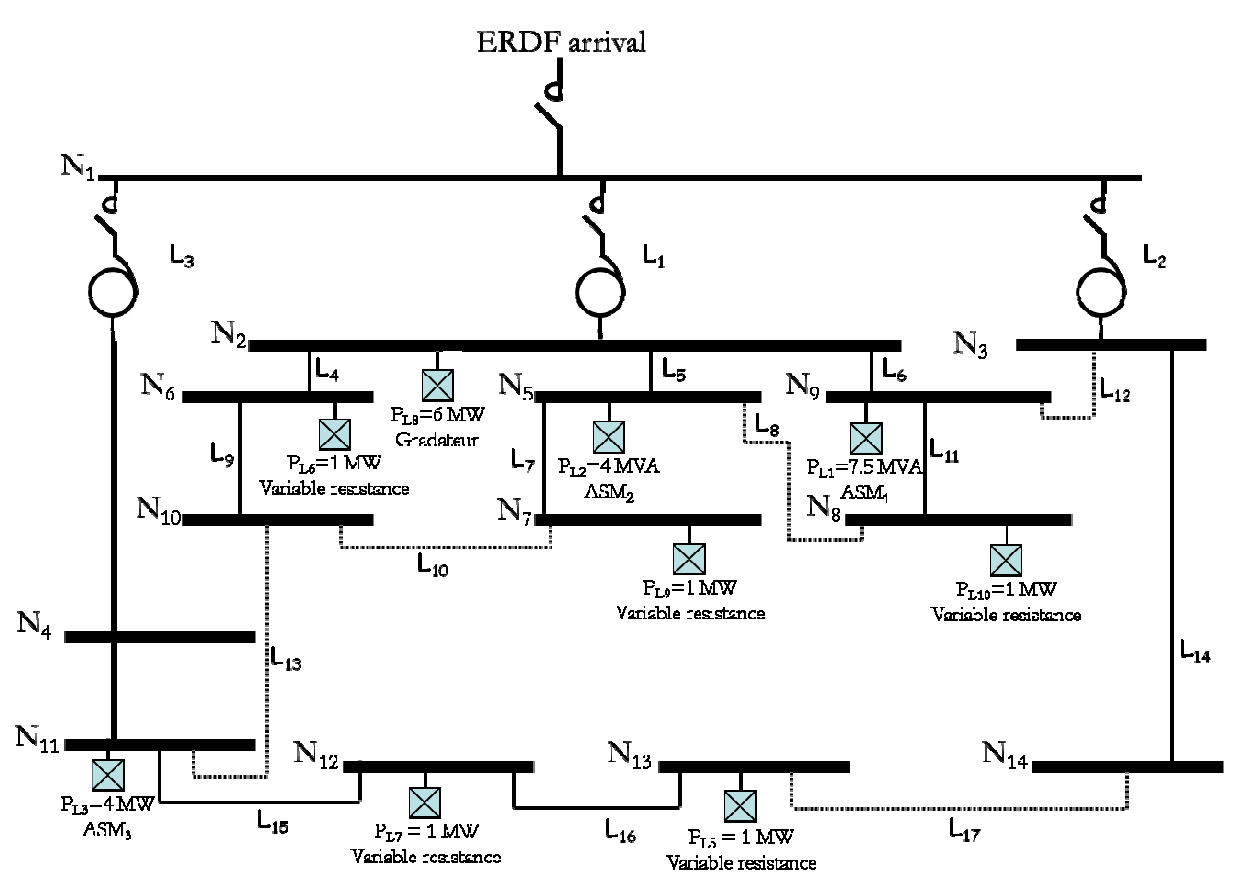
\includegraphics[width=1\textwidth]{NwImages/PREDIS}
	\captionof{figure}{The PREDIS/Urban Distribution Network}
	\labelFigure{fig:predisnw}
    \end{minipage}
    \begin{minipage}[h]{.35\textwidth }
    \centering
	\begin{tabular}{cc}
	\hline
	Voltage & $11$ kV\\
	% \hline
	\rowcolor{gray!15}
	Power & $100$ MVA\\
	% \hline
	Current &  $5248.6$ A\\
	% \hline
	\rowcolor{gray!15}
	Impedance & $1.21$ $\Omega$\\
	\hline
	\end{tabular}
	\caption{PREDIS - Base Values}
	\labelTable{predisbase}

	\vspace*{1 cm}

	\begin{tabular}{cc}
	% \hline
	\rowcolor{gray!25}
	\textbf{Lines} & \textbf{I max}\\
	\hline
	$7$, $8$, $10$ \& $11$ & $195$ A\\
	% \hline
	\rowcolor{gray!15}
	$14$ & $302$ A\\
	% \hline
	$4$, $9$ \& $15-17$ & $363$ A\\
	% \hline
	\rowcolor{gray!15}
	$6$ & $402$ A\\
	% \hline
	$5$ & $538$ A\\
	% \hline
	\rowcolor{gray!15}
	$1-3$, $12$ \& $13$ & $1$ pu\\
	\hline
	\end{tabular}
	\caption{PREDIS - $I_{max}$}
	\labelTable{predisImax}
    \end{minipage}%
\end{table}


\begin{table}[!h]
    \begin{minipage}[!h]{.5\textwidth}
	\centering
	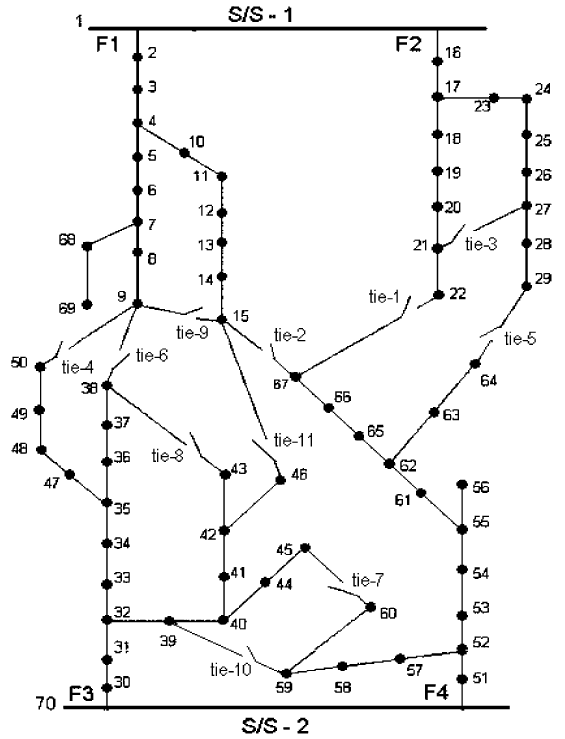
\includegraphics[width=0.8\textwidth]{NwImages/Rural_Network}
	\captionof{figure}{The Rural Distribution Network}
	\labelFigure{fig:dasnw}
    \end{minipage}
    \begin{minipage}[h]{.5\textwidth }
    \centering
	\begin{tabular}{cc}
	\hline
	Voltage & $11$ kV\\
	% \hline
	\rowcolor{gray!15}
	Power & $10$ MVA\\
	% \hline
	Current &  $524.86$ A\\
	% \hline
	\rowcolor{gray!15}
	Impedance & $12.1$ $\Omega$\\
	\hline
	\end{tabular}
	\caption{Rural Network - Base Values}
	\labelTable{dasbase}

	\vspace*{1 cm}

	\begin{tabular}{cc}
	% \hline
	\rowcolor{gray!25}
	\textbf{Lines} & \textbf{I max}\\
	\hline
	Tie Lines & $234$ A\\
	% \hline
	\rowcolor{gray!15}
	$1-18$, $17-23$ & $270$ A\\
	$31-39$, $52-57$ & $270$ A \\
	% \hline
	\rowcolor{gray!15}
	$9-16$, $24-30$ & $208$ A\\
	$40-51$, $58-68$ & $208$ A\\
	\hline
	\end{tabular}
	\caption{Rural Network - $I_{max}$}
	\labelTable{dasImax}
    \end{minipage}%
\end{table}

The two networks are varied in nature, and they were chosen with this very thought in mind. The urban network is smaller in size, with $14$ buses and $17$ lines. The rural network has $69$ buses and $79$ lines. The application of the developed algorithm to two different networks should ideally yield different results, and it would be interesting to compare and contrast them with one another.\\

The PREDIS network already has DRES connected. However, the rural network has no DRES data. Therefore, using a program developed by Marie-C\'{e}cile Alvarez-Herault\footnote{Marie-C\'{e}cile Alvarez-Herault is an associate professor at Grenoble INP, and a researcher at G2E Lab, where she works in the SYREL Team.}, DRES were randomly connected to the network for a $30\%$ insertion rate.\\

A load flow on the networks (using the applied models developed in \refSectionOnly{sec:appliedmodels}) showed that the problems associated with the two networks were indeed as thought. The urban network had many violations of current and voltage limits, while the rural network had fewer of the same.

\section {Models Applied to Test Networks}
\labelSection{sec:appliedmodels}

\lettrine[nindent=0pt]{T}{wo} load curves were created for each of the networks, based on the models explained earlier. The first one (model A) involved a simple association of one load type to each node in the networks.\\

In the second model (model B), for each node in both the test networks, a pseudo-random percentage of each of the load types was assigned. The assignment was pseudo-random in the sense that care was taken to see that the percentage of certain load types (for e.g.\ lighting) did not become unnaturally high. Typically, the load types were randomly assigned a percentage in the ranges shown in \refTableOnly{RICLperc}.\\

\begin{table}[H]
\centering
\begin{tabular}{ccc}
% \hline
\rowcolor{gray!25}
\textbf{Load Type} & \textbf{PREDIS Network} & \textbf{Rural Network}\\
\hline
Residential & $5-80$\% & $8-50$\% \\
% \hline
\rowcolor{gray!15}
Industrial & $5-50$\% & $20-75$\% \\
% \hline
Commercial & $0-50$\% & $5-70$\% \\
% \hline
\rowcolor{gray!15}
Lighting & $5-15$\% & $5-15$\% \\
\hline
\end{tabular}
\caption{Load Percentages}
\labelTable{RICLperc}
\end{table}

Based on these percentages, the two models were adapted to the two networks, and the day-ahead load curves were derived. The curves for both models are shown in \refFigureOnly{fig:dayaheadloadcurves}.\\

\begin{figure}[!h]
\begin{minipage}[!h]{.5\textwidth}
	\centering
    \setlength\figureheight{5cm}
    \setlength\figurewidth{6cm}
	% This file was created by matlab2tikz v0.4.6 running on MATLAB 8.2.
% Copyright (c) 2008--2014, Nico Schlömer <nico.schloemer@gmail.com>
% All rights reserved.
% Minimal pgfplots version: 1.3
% 
% The latest updates can be retrieved from
%   http://www.mathworks.com/matlabcentral/fileexchange/22022-matlab2tikz
% where you can also make suggestions and rate matlab2tikz.
% 
\begin{tikzpicture}

\begin{axis}[%
width=\figurewidth,
height=\figureheight,
scale only axis,
xmin=1,
xmax=24,
xtick={ 0,  4,  8, 12, 16, 20, 24},
xlabel={Time (hour)},
ymin=8,
ymax=28,
ytick={8, 12, 16, 20, 24, 28},
ylabel={Demand (MW)},
axis x line*=bottom,
axis y line*=left,
legend style={draw=black,fill=white,legend cell align=left, at={(0.5,-0.25)},anchor=north, legend columns=1}
]
\addplot [color=red,solid,mark=asterisk,mark options={solid}]
  table[row sep=crcr]{
0	13.075	\\
1	12.425	\\
2	11.2375	\\
3	11.5375	\\
4	10.6	\\
5	10.3	\\
6	11.475	\\
7	11.4625	\\
8	19.0625	\\
9	23.875	\\
10	24.6125	\\
11	24.9625	\\
12	25.5	\\
13	23.2875	\\
14	24.675	\\
15	24.475	\\
16	24.425	\\
17	23.7875	\\
18	23.325	\\
19	22.3125	\\
20	19.1375	\\
21	17.9625	\\
22	16.15	\\
23	15.5	\\
};
\addlegendentry{PREDIS Network - Model A};

\addplot [color=blue,solid,mark=+,mark options={solid}]
  table[row sep=crcr]{
0	18.496225	\\
1	17.036725	\\
2	15.260025	\\
3	16.0541	\\
4	15.161975	\\
5	14.386975	\\
6	14.802225	\\
7	13.498	\\
8	15.3973125	\\
9	17.417625	\\
10	18.01275	\\
11	18.69725	\\
12	18.995375	\\
13	17.869	\\
14	19.264625	\\
15	18.967625	\\
16	19.058125	\\
17	18.8933125	\\
18	23.422125	\\
19	24.88935	\\
20	24.3281	\\
21	23.91285	\\
22	23.380475	\\
23	21.920975	\\
};
\addlegendentry{PREDIS Network - Model B};

\end{axis}
\end{tikzpicture}%
\end{minipage}
\begin{minipage}[!h]{.5\textwidth}
	\centering
	\setlength\figureheight{5cm}
    \setlength\figurewidth{6cm}
	% This file was created by matlab2tikz v0.4.6 running on MATLAB 8.2.
% Copyright (c) 2008--2014, Nico Schlömer <nico.schloemer@gmail.com>
% All rights reserved.
% Minimal pgfplots version: 1.3
% 
% The latest updates can be retrieved from
%   http://www.mathworks.com/matlabcentral/fileexchange/22022-matlab2tikz
% where you can also make suggestions and rate matlab2tikz.
% 
\begin{tikzpicture}

\begin{axis}[%
width=\figurewidth,
height=\figureheight,
scale only axis,
xmin=1,
xmax=24,
xtick={ 0,  4,  8, 12, 16, 20, 24},
xlabel={Time (hour)},
ymin=1,
ymax=4,
ylabel={Demand (MW)},
axis x line*=bottom,
axis y line*=left,
legend style={draw=black,fill=white,legend cell align=left, at={(0.5,-0.25)},anchor=north, legend columns=1}
]

\addplot [color=red,solid,mark=triangle,mark options={solid}]
  table[row sep=crcr]{
0	2.349405	\\
1	2.20301	\\
2	2.042415	\\
3	1.99943	\\
4	1.99943	\\
5	1.95381	\\
6	2.00256	\\
7	2.59775	\\
8	1.699105	\\
9	1.8097	\\
10	2.518825	\\
11	2.59002	\\
12	2.384425	\\
13	2.64015	\\
14	2.469825	\\
15	1.85725	\\
16	2.234675	\\
17	2.170975	\\
18	3.533	\\
19	3.68714	\\
20	3.785935	\\
21	3.54921	\\
22	3.187735	\\
23	2.725685	\\
};
\addlegendentry{Rural Network - Model A};

\addplot [color=blue,solid,mark=square,mark options={solid}]
  table[row sep=crcr]{
0	2.05807563	\\
1	1.7963816	\\
2	1.57114753	\\
3	1.51164628	\\
4	1.51164628	\\
5	1.42596326	\\
6	1.47316896	\\
7	2.22160334	\\
8	1.91887959	\\
9	2.25947876	\\
10	2.86462259	\\
11	2.87541732	\\
12	2.67237475	\\
13	2.8661525	\\
14	2.84984517	\\
15	2.2010163	\\
16	2.69893055	\\
17	2.56839365	\\
18	3.556118	\\
19	3.66603836	\\
20	3.80485395	\\
21	3.65398318	\\
22	3.28427879	\\
23	2.68812165	\\
};
\addlegendentry{Rural Network - Model B};

\end{axis}
\end{tikzpicture}%
\end{minipage}
\caption{Day-ahead Load Curves (Models A \& B) for the Test Networks}
\labelFigure{fig:dayaheadloadcurves}
\end{figure}

As for the DRES production, the cumulative values are shown in \refFigureOnly{fig:dayaheadDREScurves}.\\

\begin{figure}[!h]
\begin{minipage}[!h]{.5\textwidth}
	\centering
    \setlength\figureheight{5cm}
    \setlength\figurewidth{6cm}
	% This file was created by matlab2tikz v0.4.6 running on MATLAB 8.2.
% Copyright (c) 2008--2014, Nico Schlömer <nico.schloemer@gmail.com>
% All rights reserved.
% Minimal pgfplots version: 1.3
% 
% The latest updates can be retrieved from
%   http://www.mathworks.com/matlabcentral/fileexchange/22022-matlab2tikz
% where you can also make suggestions and rate matlab2tikz.
% 
\begin{tikzpicture}

\begin{axis}[%
width=\figurewidth,
height=\figureheight,
scale only axis,
xmin=1,
xmax=24,
xlabel={Time (hour)},
ymin=0,
ymax=16,
ylabel={Production (MW)},
axis x line*=bottom,
axis y line*=left,
legend style={draw=black,fill=white,legend cell align=left, at={(0.5,-0.25)},anchor=north, legend columns=1}
]
\addplot [color=blue,solid]
  table[row sep=crcr]{
0	3.852	\\
1	5.728	\\
2	5.338	\\
3	4.864	\\
4	1.707	\\
5	2.045	\\
6	1.749	\\
7	0.532	\\
8	1.006	\\
9	8.0293793	\\
10	7.3152759	\\
11	11.8102414	\\
12	15.528	\\
13	9.4014483	\\
14	13.7370345	\\
15	10.3953103	\\
16	5.206	\\
17	1.792	\\
18	7.956	\\
19	3.652	\\
20	3.417	\\
21	6.016	\\
22	0.514	\\
23	8.088	\\
};
\addlegendentry{PREDIS Network};

\end{axis}
\end{tikzpicture}%
\end{minipage}
\begin{minipage}[!h]{.5\textwidth}
	\centering
	\setlength\figureheight{5cm}
    \setlength\figurewidth{6cm}
	% This file was created by matlab2tikz v0.4.6 running on MATLAB 8.2.
% Copyright (c) 2008--2014, Nico Schlömer <nico.schloemer@gmail.com>
% All rights reserved.
% Minimal pgfplots version: 1.3
% 
% The latest updates can be retrieved from
%   http://www.mathworks.com/matlabcentral/fileexchange/22022-matlab2tikz
% where you can also make suggestions and rate matlab2tikz.
% 
\begin{tikzpicture}

\begin{axis}[%
width=\figurewidth,
height=\figureheight,
scale only axis,
xmin=1,
xmax=24,
xlabel={Time (hour)},
ymin=0.8,
ymax=2,
ylabel={Production (MW)},
axis x line*=bottom,
axis y line*=left,
legend style={draw=black,fill=white,legend cell align=left, at={(0.5,-0.25)},anchor=north, legend columns=1}
]
\addplot [color=red,solid]
  table[row sep=crcr]{
0	1.3204366	\\
1	1.58013391	\\
2	1.67322503	\\
3	1.99318176	\\
4	1.4954867	\\
5	1.66521042	\\
6	1.43650239	\\
7	1.62284984	\\
8	1.60521016	\\
9	1.68773886	\\
10	1.51032673	\\
11	0.90721418	\\
12	1.61214652	\\
13	1.8977162	\\
14	1.95117643	\\
15	1.5312021	\\
16	1.76392663	\\
17	1.5445812	\\
18	1.98685491	\\
19	1.80166541	\\
20	1.5223008	\\
21	1.59099695	\\
22	1.76961399	\\
23	1.44837906	\\
};
\addlegendentry{Rural Network};

\end{axis}
\end{tikzpicture}%
\end{minipage}
\caption{Cumulative Day-ahead DRES Production Curves for the Test Networks}
\labelFigure{fig:dayaheadDREScurves}
\end{figure}

The curves show a major share of power coming from solar energy in the PREDIS network (understandably, given that it is an urban network) and a major share for wind power in the rural network (evident with a dip during midday, something that would have normally not happened with solar power). These are the models that have been utilized for the algorithm.\\

For the two networks, the maximum insertion rate of DRES is shown below. The values change every hour for both the networks.

\begin{table}[h]
\centering
\begin{tabular}{ccc}
% \hline
\rowcolor{gray!25}
& \textbf{Load Model A} & \textbf{Load Model B}\\
\hline
PREDIS Network & $60.89$\% (Hour $12$) & $81.75$\% (Hour $12$) \\
% \hline
\rowcolor{gray!15}
Rural Network & $99.69$\% (Hour $3$) & $131.86$\% (Hour $3$) \\
\hline
\end{tabular}
\caption{DRES Insertion Rates}
\labelTable{dresins}
\end{table}

In the case where the insertion rate is higher than $100$\%, there is a possibility for injection of power from the distribution network to the transmission network. This is unadvisable and causes other constraints, which will be treated in due course of development.


